%%%%%%%%%%%%%%%%%%%%%%%%%%%%%%%%%%%%%%%%%
% Programming/Coding Assignment
% LaTeX Template
%
% This template has been downloaded from:
% http://www.latextemplates.com
%
% Original author:
% Ted Pavlic (http://www.tedpavlic.com)
%
% Note:
% The \lipsum[#] commands throughout this template generate dummy text
% to fill the template out. These commands should all be removed when 
% writing assignment content.
%
% This template uses a Perl script as an example snippet of code, most other
% languages are also usable. Configure them in the "CODE INCLUSION 
% CONFIGURATION" section.
%
%%%%%%%%%%%%%%%%%%%%%%%%%%%%%%%%%%%%%%%%%

%----------------------------------------------------------------------------------------
%	PACKAGES AND OTHER DOCUMENT CONFIGURATIONS
%----------------------------------------------------------------------------------------

\documentclass{article}

\usepackage[utf8]{inputenc}
\usepackage{fancyhdr} % Required for custom headers
\usepackage{lastpage} % Required to determine the last page for the footer
\usepackage{extramarks} % Required for headers and footers
\usepackage[usenames,dvipsnames]{color} % Required for custom colors
\usepackage{graphicx} % Required to insert images
\usepackage{listings} % Required for insertion of code
\usepackage{courier} % Required for the courier font
\usepackage{lipsum} % Used for inserting dummy 'Lorem ipsum' text into the template

% Margins
\topmargin=-0.45in
\evensidemargin=0in
\oddsidemargin=0in
\textwidth=6.5in
\textheight=9.0in
\headsep=0.25in

\linespread{1.1} % Line spacing

% Set up the header and footer
\pagestyle{fancy}
\lhead{\hmwkAuthorName} % Top left header
\chead{\hmwkClass\ (\hmwkClassInstructor\ \hmwkClassTime): \hmwkTitle} % Top center head
\rhead{\firstxmark} % Top right header
\lfoot{\lastxmark} % Bottom left footer
\cfoot{} % Bottom center footer
\rfoot{Page\ \thepage\ of\ \protect\pageref{LastPage}} % Bottom right footer
\renewcommand\headrulewidth{0.4pt} % Size of the header rule
\renewcommand\footrulewidth{0.4pt} % Size of the footer rule

\setlength\parindent{0pt} % Removes all indentation from paragraphs

%----------------------------------------------------------------------------------------
%	CODE INCLUSION CONFIGURATION
%----------------------------------------------------------------------------------------

\definecolor{MyDarkGreen}{rgb}{0.0,0.4,0.0} % This is the color used for comments
\lstloadlanguages{Perl} % Load Perl syntax for listings, for a list of other languages supported see: ftp://ftp.tex.ac.uk/tex-archive/macros/latex/contrib/listings/listings.pdf
\lstset{language=Perl, % Use Perl in this example
        frame=single, % Single frame around code
        basicstyle=\small\ttfamily, % Use small true type font
        keywordstyle=[1]\color{Blue}\bf, % Perl functions bold and blue
        keywordstyle=[2]\color{Purple}, % Perl function arguments purple
        keywordstyle=[3]\color{Blue}\underbar, % Custom functions underlined and blue
        identifierstyle=, % Nothing special about identifiers                                         
        commentstyle=\usefont{T1}{pcr}{m}{sl}\color{MyDarkGreen}\small, % Comments small dark green courier font
        stringstyle=\color{Purple}, % Strings are purple
        showstringspaces=false, % Don't put marks in string spaces
        tabsize=5, % 5 spaces per tab
        %
        % Put standard Perl functions not included in the default language here
        morekeywords={rand},
        %
        % Put Perl function parameters here
        morekeywords=[2]{on, off, interp},
        %
        % Put user defined functions here
        morekeywords=[3]{test},
       	%
        morecomment=[l][\color{Blue}]{...}, % Line continuation (...) like blue comment
        numbers=left, % Line numbers on left
        firstnumber=1, % Line numbers start with line 1
        numberstyle=\tiny\color{Blue}, % Line numbers are blue and small
        stepnumber=5 % Line numbers go in steps of 5
}

% Creates a new command to include a perl script, the first parameter is the filename of the script (without .pl), the second parameter is the caption
\newcommand{\perlscript}[2]{
\begin{itemize}
\item[]\lstinputlisting[caption=#2,label=#1]{#1.pl}
\end{itemize}
}

%----------------------------------------------------------------------------------------
%	DOCUMENT STRUCTURE COMMANDS
%	Skip this unless you know what you're doing
%----------------------------------------------------------------------------------------

% Header and footer for when a page split occurs within a problem environment
\newcommand{\enterProblemHeader}[1]{
\nobreak\extramarks{#1}{#1 continued on next page\ldots}\nobreak
\nobreak\extramarks{#1 (continued)}{#1 continued on next page\ldots}\nobreak
}

% Header and footer for when a page split occurs between problem environments
\newcommand{\exitProblemHeader}[1]{
\nobreak\extramarks{#1 (continued)}{#1 continued on next page\ldots}\nobreak
\nobreak\extramarks{#1}{}\nobreak
}

\setcounter{secnumdepth}{0} % Removes default section numbers
\newcounter{homeworkProblemCounter} % Creates a counter to keep track of the number of problems

\newcommand{\homeworkProblemName}{}
\newenvironment{homeworkProblem}[1][Task \arabic{homeworkProblemCounter}]{ % Makes a new environment called homeworkProblem which takes 1 argument (custom name) but the default is "Problem #"
\stepcounter{homeworkProblemCounter} % Increase counter for number of problems
\renewcommand{\homeworkProblemName}{#1} % Assign \homeworkProblemName the name of the problem
\section{\homeworkProblemName} % Make a section in the document with the custom problem count
\enterProblemHeader{\homeworkProblemName} % Header and footer within the environment
}{
\exitProblemHeader{\homeworkProblemName} % Header and footer after the environment
}

\newcommand{\problemAnswer}[1]{ % Defines the problem answer command with the content as the only argument
\noindent\framebox[\columnwidth][c]{\begin{minipage}{0.98\columnwidth}#1\end{minipage}} % Makes the box around the problem answer and puts the content inside
}

\newcommand{\homeworkSectionName}{}
\newenvironment{homeworkSection}[1]{ % New environment for sections within homework problems, takes 1 argument - the name of the section
\renewcommand{\homeworkSectionName}{#1} % Assign \homeworkSectionName to the name of the section from the environment argument
\subsection{\homeworkSectionName} % Make a subsection with the custom name of the subsection
\enterProblemHeader{\homeworkProblemName\ [\homeworkSectionName]} % Header and footer within the environment
}{
\enterProblemHeader{\homeworkProblemName} % Header and footer after the environment
}

%----------------------------------------------------------------------------------------
%	NAME AND CLASS SECTION
%----------------------------------------------------------------------------------------

\newcommand{\hmwkTitle}{Report\ \#1} % Assignment title
\newcommand{\hmwkDueDate}{Monday,\ May\ 5,\ 2014} % Due date
\newcommand{\hmwkClass}{INEA00104L} % Course/class
\newcommand{\hmwkClassTime}{} % Class/lecture time
\newcommand{\hmwkClassInstructor}{Mgr inż. Andrzej Wytyczak-Partyka} % Teacher/lecturer
\newcommand{\hmwkAuthorName}{inż. Piotr Giedziun} % Your name

%----------------------------------------------------------------------------------------
%	TITLE PAGE
%----------------------------------------------------------------------------------------

\title{
\vspace{2in}
\textmd{\textbf{\hmwkClass:\ \hmwkTitle}}\\
\normalsize\vspace{0.1in}\small{Due\ on\ \hmwkDueDate}\\
\vspace{0.1in}\large{\textit{\hmwkClassInstructor\ \hmwkClassTime}}
\vspace{3in}
}

\author{\textbf{\hmwkAuthorName}}
\date{} % Insert date here if you want it to appear below your name

%----------------------------------------------------------------------------------------

\begin{document}

\maketitle

%----------------------------------------------------------------------------------------
%	TABLE OF CONTENTS
%----------------------------------------------------------------------------------------

%\setcounter{tocdepth}{1} % Uncomment this line if you don't want subsections listed in the ToC

\newpage
\tableofcontents
\newpage


\section{Introduction}
This report was made to present results of work made during third laboratory.
Main goal of this lab was to introduce basic optimization topics.
Performed tasks focused on indexes usage.
Without an index, would begin with the first row and then read through the entire table to find the relevant rows. 
Indexes allow to improve performance on aspects like WHERE clause, finding MIN/MAX, sorting etc.
\newline\newline
Database schema used in this lab was based on previous labs.
We were asked to create database for cinema. This topic includes usage of triggers, views and basics of relational databases.

\section{Database}
In order to perform given task, we had to add additional field - \textbf{theater\_id} (type of INT).
Figure \ref{fig:database} shows changes made to \textbf{ticket} table. Filed \textbf{theater\_id} is just normal field (it's not liked as a foreign key).

\begin{figure}[ht!]
\centering
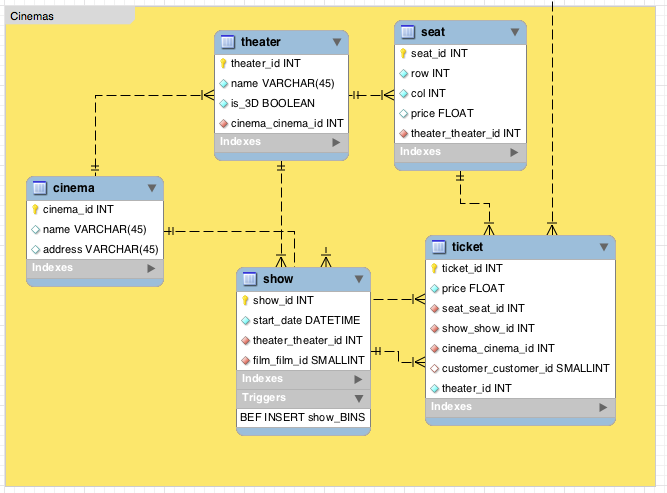
\includegraphics[width=0.75\columnwidth]{database} 
\caption{Part of database EER Diagram}
\label{fig:database}
\end{figure}

%----------------------------------------------------------------------------------------
%	TASK 1
%----------------------------------------------------------------------------------------

\begin{homeworkProblem}
First task was to create SELECT query with WHERE clause on \textbf{ticket.theater\_id} field.
Another part of the task was to study performance of query WITH/WITHOUT index on \textbf{ticket.theater\_id}.
\newline\newline
Following query adds INDEX on theater\_id.
\begin{lstlisting}[language=SQL] 
CREATE INDEX theater_id_index ON `ticket` (theater_id) USING BTREE;
\end{lstlisting}

Following query was used to measure performance time.	
\begin{lstlisting}[language=SQL] 
SELECT SQL_NO_CACHE * FROM `ticket` WHERE theater_id = 3;
\end{lstlisting}

\subsection{Query WITHOUT index on theater\_id}

First step I did was to use EXPLAIN statement. The EXPLAIN statement provides information about how MySQL executes statements.

\begin{lstlisting}[language=SQL] 
EXPLAIN SELECT * FROM `ticket` WHERE theater_id = 3; 

id,select_type,table,type,possible_keys,key,key_len,ref,rows,Extra
1,SIMPLE,ticket,ALL,NULL,NULL,NULL,NULL,99814,"Using where"
\end{lstlisting}

In order to obtain results under hood MySQL is looking through all rows. Field "rows" is equals to number of rows in ticket table.
This approach is not optimal, it will be dependent on rows count.

\subsection{Query WITH index on theater\_id}
\begin{lstlisting}[language=SQL] 
EXPLAIN SELECT * FROM `ticket` WHERE theater_id = 3;

id,select_type,table,type,possible_keys,key,key_len,ref,rows,Extra
1,SIMPLE,ticket,ref,theater_id,theater_id,4,const,100,NULL
\end{lstlisting}

In this case MySQL is looking through only 100 rows. This result was achieved thanks to B-tree construction of index table.

\subsection{Results}

As expected there is a huge spike between execution with and without index on theater\_id.
For smaller instances (like 1k) execution time was similar. It's wasn't the case for 10k+ rows.
\newline\newline
Results presented in table.
\begin{center}
\begin{tabular}{ l | r | r | r | r }
  & 1k & 10k & 100k & 1000k \\
  with & 0.07s & 0.064s & 0.066s & 0.073s \\
  without & 0.09s & 0.433s & 3.6s & 37.02s \\
\end{tabular}
\end{center}

Results presented as line chart.

\begin{figure}[ht!]
\centering
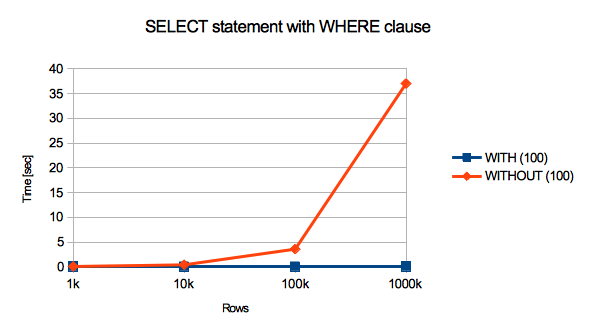
\includegraphics[width=0.60\columnwidth]{select_where_results} 
\caption{SELECT statement with WHERE clause}
\label{fig:task1result}
\end{figure}

\end{homeworkProblem}

%----------------------------------------------------------------------------------------
%	PROBLEM 2
%----------------------------------------------------------------------------------------

\begin{homeworkProblem}
Second task was also to determine difference between using/not using index on start\_date field.
This time on DATE field. Date fields behave similar to integer fields, so expected graph should be similar to presented in first task.
\newline\newline
Following query was used to measure performance time.	
\begin{lstlisting}[language=SQL] 
SELECT 
    ti . *, sh.start_date
FROM
    `ticket` ti
        INNER JOIN
    `show` sh ON ti.show_show_id = sh.show_id
WHERE
    start_date > now()
        AND start_date < DATE_ADD(now(), INTERVAL 1 YEAR);
\end{lstlisting}

\subsection{Query WITHOUT index on start\_date}

First step I did was to use EXPLAIN statement. The EXPLAIN statement provides information about how MySQL executes statements.

\begin{lstlisting}[language=SQL] 
EXPLAIN SELECT COUNT(*) FROM `ticket` ti INNER JOIN `show` sh ON
 ti.show_show_id = sh.show_id WHERE start_date > now()
 AND start_date < DATE_ADD(now(), INTERVAL 1 YEAR);
\end{lstlisting}

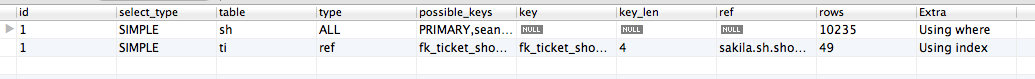
\includegraphics[width=1\columnwidth]{explain_without_date} 

There is nothing more to say here. It's the same as in previous task. 

\subsection{Query WITH index on start\_date}
\begin{lstlisting}[language=SQL] 
EXPLAIN SELECT COUNT(*) FROM `ticket` ti INNER JOIN `show` sh ON
 ti.show_show_id = sh.show_id WHERE start_date > now()
 AND start_date < DATE_ADD(now(), INTERVAL 1 YEAR);
\end{lstlisting}

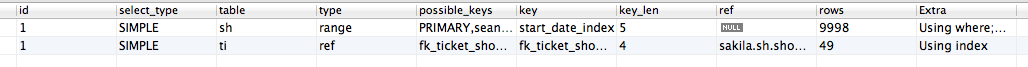
\includegraphics[width=1\columnwidth]{explain_with_date} 

Size of checked records is significantly bigger in comparison to task 1.
It's because almost all shows were played in 1 year gap.

\subsection{Results}

This time around I have received almost identical results for both cases. It's because almost all shows were played in 1 year gap.
\newline\newline
Results presented in table.

\begin{center}
\begin{tabular}{ l | r | r | r | r }
  & 1k & 10k & 100k & 1000k \\
  with & 0.001s & 0.003s & 0.025s & 0.287s \\
  without & 0.001s & 0.003s &0.026s & 0.291s \\
\end{tabular}
\end{center}

Results presented as line chart.

\begin{figure}[ht!]
\centering
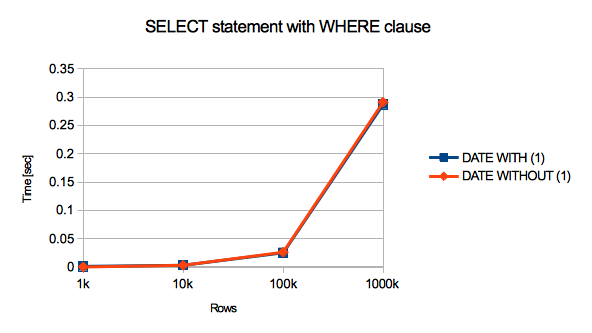
\includegraphics[width=0.60\columnwidth]{date_result} 
\caption{SELECT statement with WHERE clause}
\label{fig:task1result}
\end{figure}

\end{homeworkProblem}

%----------------------------------------------------------------------------------------
%	PROBLEM 3
%----------------------------------------------------------------------------------------

\begin{homeworkProblem}
Third task was also to determine difference between using/not using index on title field.
This time on VARCHAR field. In addition this task was divided into two smaller parts (starting with "the" and having the word "the")
\newline\newline
Following query was used to measure performance time for starting with "the".
\begin{lstlisting}[language=SQL] 
SELECT SQL_NO_CACHE
    fi.title
FROM
    `ticket` ti
        INNER JOIN
    `show` sh ON sh.show_id = ti.show_show_id
        LEFT JOIN
    `film` fi ON fi.film_id = sh.film_film_id
WHERE
    fi.title LIKE 'the%'
\end{lstlisting}

Following query was used to measure performance time for having the word "the".
\begin{lstlisting}[language=SQL] 
SELECT SQL_NO_CACHE
    fi.title
FROM
    `ticket` ti
        INNER JOIN
    `show` sh ON sh.show_id = ti.show_show_id
        LEFT JOIN
    `film` fi ON fi.film_id = sh.film_film_id
WHERE
    fi.title LIKE '%the%'
\end{lstlisting}

\subsection{Query WITHOUT index on title}

First step I did was to use EXPLAIN statement. The EXPLAIN statement provides information about how MySQL executes statements.

\begin{lstlisting}[language=SQL] 
EXPLAIN SELECT SQL_NO_CACHE fi.title FROM `ticket` ti INNER JOIN `show` sh ON
sh.show_id = ti.show_show_id LEFT JOIN `film` fi ON fi.film_id = sh.film_film_id 
WHERE fi.title LIKE '%the%'
\end{lstlisting}

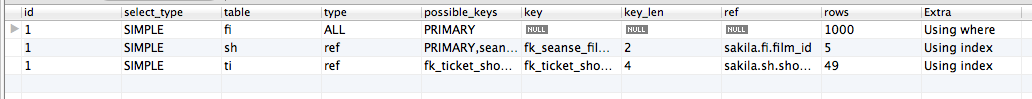
\includegraphics[width=1\columnwidth]{explain_without_text} 

\subsection{Query WITH index on title}

\begin{lstlisting}[language=SQL] 
EXPLAIN SELECT SQL_NO_CACHE fi.title FROM `ticket` ti INNER JOIN `show` sh ON
sh.show_id = ti.show_show_id LEFT JOIN `film` fi ON fi.film_id = sh.film_film_id 
WHERE fi.title LIKE '%the%'
\end{lstlisting}

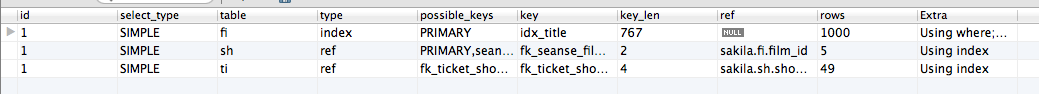
\includegraphics[width=1\columnwidth]{explain_with_text} 

\subsection{Results}
In my case film database in negligible compared to ticket size. This fact have big impact on result graph.
There is no major difference for table with 100 rows with/without indexes.\newline
In this case results were impacted by ticket table size (amount of inner joins).\newline
The main difference is that "the\%" is using indexing, unlike "\%the\%".
\newline\newline
Better example of this difference is expressed by following query.
\begin{lstlisting}[language=SQL] 
EXPLAIN SELECT * FROM sakila.film WHERE title LIKE "the%";
id,select_type,table,type,possible_keys,key,key_len,ref,rows,Extra
1,SIMPLE,film,range,idx_title,idx_title,767,NULL,1,"Using index condition"
\end{lstlisting}
It's using index condition instead of WHERE.
\begin{lstlisting}[language=SQL] 
EXPLAIN SELECT * FROM sakila.film WHERE title LIKE "%the%";
id,select_type,table,type,possible_keys,key,key_len,ref,rows,Extra
1,SIMPLE,film,ALL,NULL,NULL,NULL,NULL,1000,"Using where"
\end{lstlisting}
In this case we are looping through entire table data.
\newpage
Results presented as line chart.

\begin{figure}[ht!]
\centering
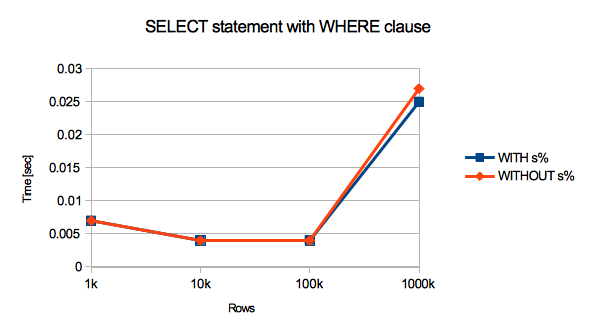
\includegraphics[width=0.70\columnwidth]{string_report_start} 
\caption{SELECT statement with WHERE clause}
\label{fig:task1result}
\end{figure}

\begin{figure}[ht!]
\centering
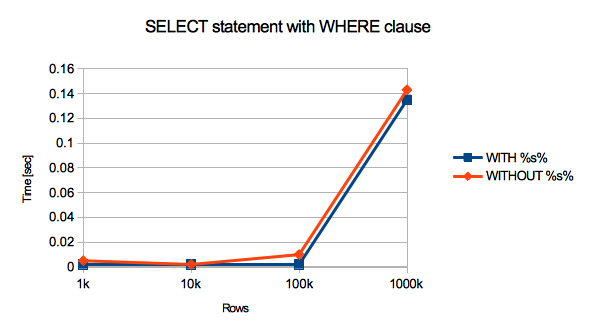
\includegraphics[width=0.70\columnwidth]{string_report_having} 
\caption{SELECT statement with WHERE clause}
\label{fig:task1result}
\end{figure}

\end{homeworkProblem}

\section{Summary}

\begin{itemize}
  \item All indexes in our tasks (data types - INT, VARCHAR, DATA) were stored in B-trees.
  \item For those task, where number of searches records were about 10k+ there were huge performance improvement for those with index.
  \item It's always good practice to use indexes while creating database model.
  \item Indexes should be created on fields used in WHERE clause, finding  MIN/MAX and sorting.
\end{itemize}

\section{Webpage}
Part of laboratory preparation was to create website to handle requests. Prepared site is able to display movies list, cinemas list, view upcoming show and book seats.

\begin{figure}[ht!]
\centering
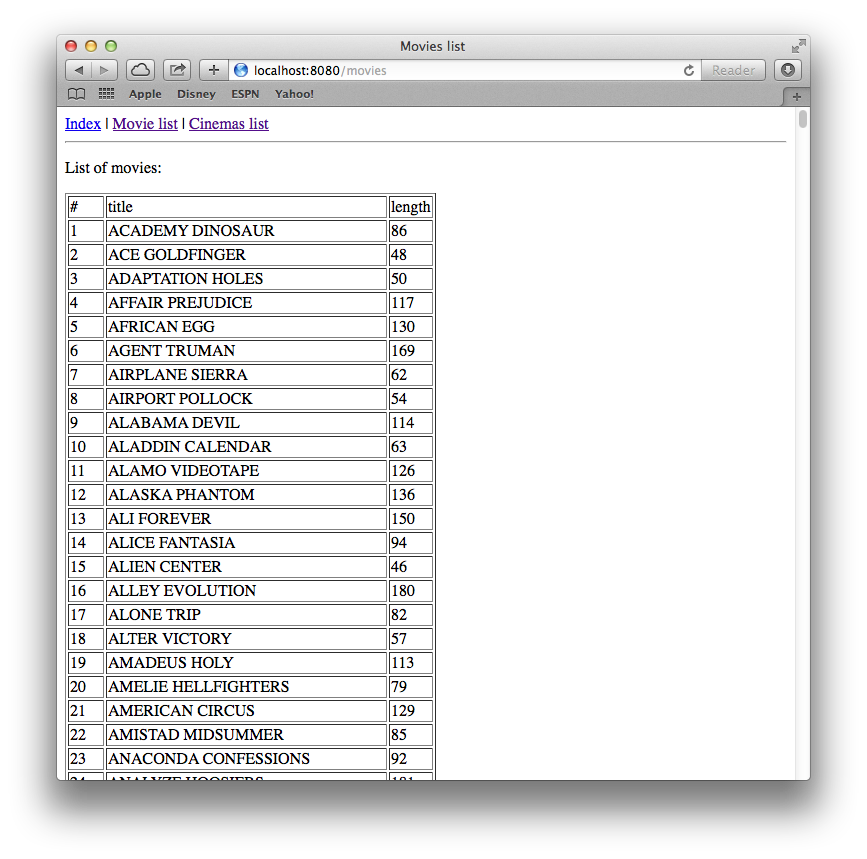
\includegraphics[width=0.60\columnwidth]{www_ss1} 
\caption{Movies list}
\end{figure}

\begin{figure}[ht!]
\centering
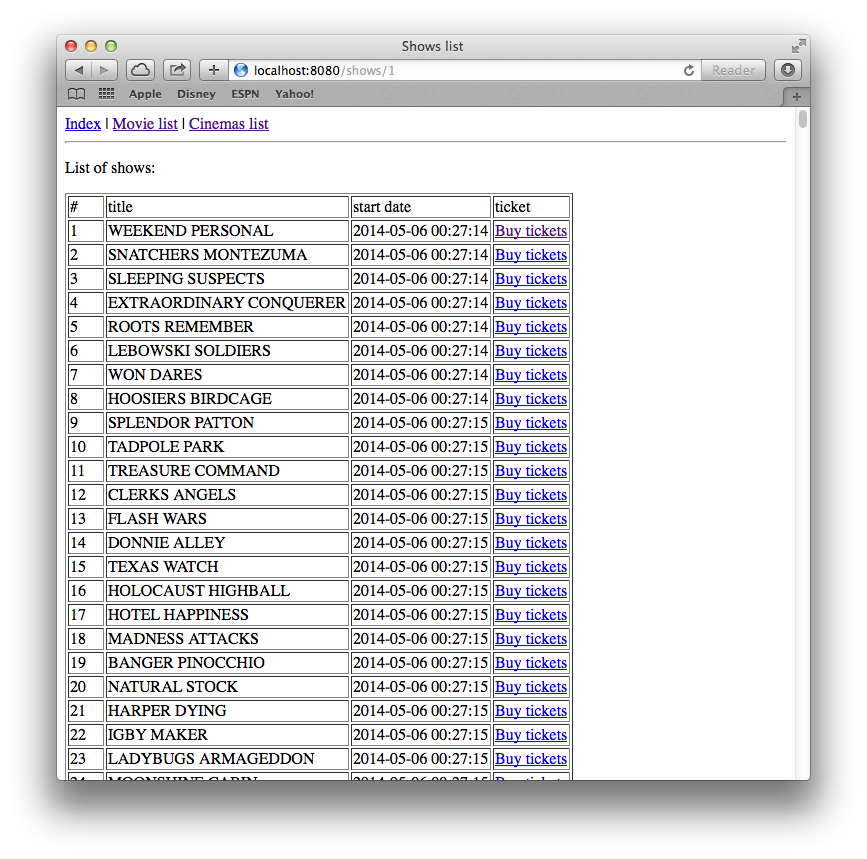
\includegraphics[width=0.60\columnwidth]{www_ss2} 
\caption{Shows list}
\end{figure}

\begin{figure}[ht!]
\centering
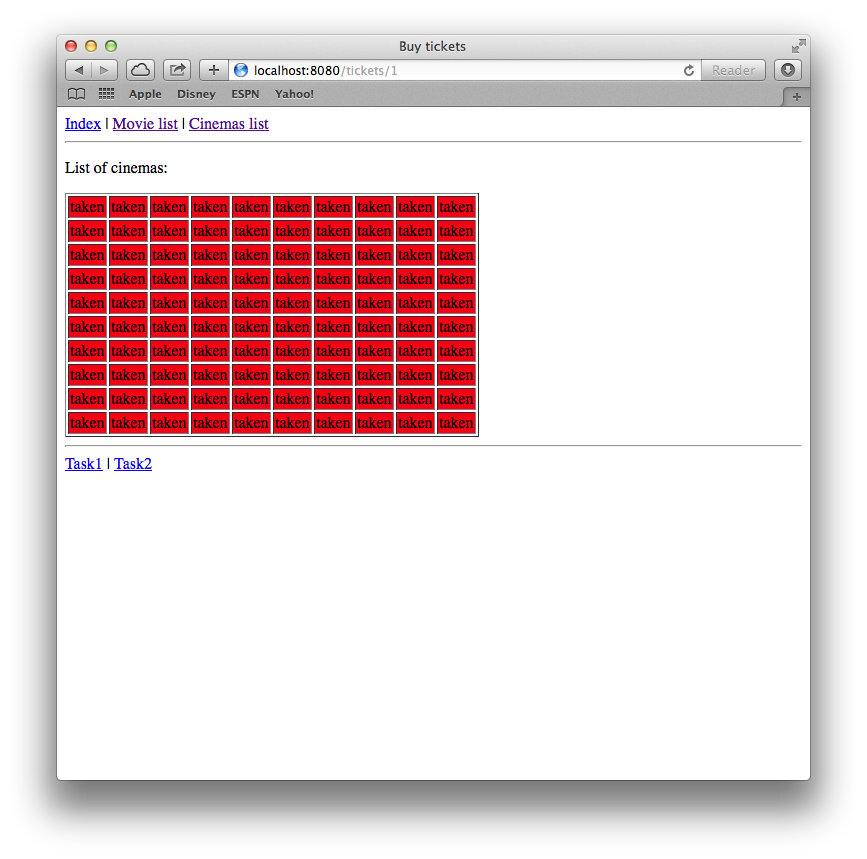
\includegraphics[width=0.60\columnwidth]{www_ss3} 
\caption{Seats for selected show}
\end{figure}

\end{document}